\documentclass{beamer}
\usetheme{default}
\beamertemplatenavigationsymbolsempty
\usepackage{rembeamer}

\begin{document}

\begin{frame}
  \frametitle{Title}
  \begin{itemize}
    \item[] 
    Conducting hypothesis testing for difference in categorical
    variables with more than two levels and interpreting the results. 
  \end{itemize}
\end{frame}

\begin{frame}
  \frametitle{Contingency (Two-Way) Table}
  \begin{table}
    \begin{tabular}{@{}cccc@{}}
      \toprule
      & Sun & Partial Shade & Shade \\
      \cmidrule(r){1-1} \cmidrule(rl){2-2} \cmidrule(rl){3-3}
      \cmidrule(l){4-4}
      Desert & 16 & 32 & 71 \\[0.3em]
      Valley & 42 & 40 & 24 \\[0.3em]
      Mountain & 56 & 36 & 15 \\
      \bottomrule
    \end{tabular}
  \end{table}
\end{frame}

\begin{frame}
  \frametitle{Psychology Study on Purchasing Questions}
  \begin{itemize}
    \item[] 
      219 sellers and 219 potential buyers.
      \vspace{0.5cm}
    \item[] 
      Possible defective iPod (two freezes in its history). 
      \vspace{0.5cm}
    \item[] 
      What can you tell me about it?
      \vspace{0.5cm}
    \item[] 
      It doesn't have any problems, does it?
      \vspace{0.5cm}
    \item[] 
      What problems does it have?
  \end{itemize}
\end{frame}

\begin{frame}
  \frametitle{Contingency Table}
  \begin{table}
    \begin{tabular}{@{}cccc@{}}
      \toprule
      Question & Disclose & Hide & Total \\
      \cmidrule(r){1-1} \cmidrule(rl){2-2} \cmidrule(rl){3-3}
      \cmidrule(l){4-4}
      Neutral & 2 & 71 & 73 \\[0.3em]
      Positive & 23 & 50 & 73 \\[0.3em]
      Negative & 36 & 37 & 73 \\
      Total & 61 & 36 & 219 \\
      \bottomrule
    \end{tabular}
  \end{table}
\end{frame}

\begin{frame}
  \frametitle{Contingency Table}
  \begin{table}
    \begin{tabular}{@{}cccc@{}}
      \toprule
      Question & Disclose & Hide & Total \\
      \cmidrule(r){1-1} \cmidrule(rl){2-2} \cmidrule(rl){3-3}
      \cmidrule(l){4-4}
      Neutral & 2 & 71 & 73 \\[0.3em]
      Positive & 23 & 50 & 73 \\[0.3em]
      Negative & 36 & 37 & 73 \\
      Total & 61 & 36 & 219 \\
      \bottomrule
    \end{tabular}
  \end{table}
  \begin{equation*}
    \frac{2 + 23 + 36}{219} = 0.278 \hspace{1cm} 0.278(73) = 20.33
  \end{equation*}
  \begin{equation*}
    73 - 20.33 = 52.67 
  \end{equation*}
\end{frame}

\begin{frame}
  \frametitle{$X$-squared}
  \begin{displaymath}
    \begin{array}{lll}
      \text{Neutral-Disclose} & \frac{(2 - 20.33)^2}{20.33} & = 16.53
      \\[0.5em]
      \text{Positive-Disclose} & \frac{(23 - 20.33)^2}{20.33} & = 0.35
      \\[0.5em]
      \text{Negative-Disclose} & \frac{(36 - 20.33)^2}{20.33} & =
      12.08 \\[0.5em]
      \text{Neutral-Hide} & \frac{(71 - 52.67)^2}{52.67} & = 6.38
      \\[0.5em]
      \text{Positive-Hide} & \frac{(50 - 52.67)^2}{52.67} & = 0.14
      \\[0.5em]
      \text{Negative-Hide} & \frac{(37 - 52.67)^2}{52.67} & = 4.66
    \end{array}
  \end{displaymath}
  \begin{equation*}
    X^2 = 16.53 + 0.35 + 12.08 + 6.38 + 0.14 + 4.66 = 40.13
  \end{equation*}
\end{frame}

\begin{frame}
  \frametitle{Randomization Process}
  \begin{table}
    \begin{tabular}{@{}cccc@{}}
      \toprule
      Question & Disclose & Hide & Total \\
      \cmidrule(r){1-1} \cmidrule(rl){2-2} \cmidrule(rl){3-3}
      \cmidrule(l){4-4}
      Neutral & 2 & 71 & 73 \\[0.3em]
      Positive & 23 & 50 & 73 \\[0.3em]
      Negative & 36 & 37 & 73 \\
      Total & 61 & 36 & 219 \\
      \bottomrule
    \end{tabular}
  \end{table}
  \begin{itemize}
    \item[] 
      Shuffle the data: take the 61 disclose and 158 hide and
      re-destribute them among the groups. 
      \vspace{0.5cm}
    \item[] 
      Recalculate the $X^2$.
      \vspace{0.5cm}
    \item[] 
      Repeat many times to get a distribution. Compare the
      distribution with the sample statistics. 
  \end{itemize}
\end{frame}

\begin{frame}
  \frametitle{$X^2$ Distribution}
  \centering
  \begin{tikzpicture}
    \begin{axis}[
      xlabel={$X^2$ test statistics of random samples},
      ylabel={Count}
    ]
      \addplot+ [
        hist={bins=5},
        fill=orange,
        draw=black,
        mark=none
      ]
      table [y index=0] {../data/chisquared.csv};
    \end{axis}
  \end{tikzpicture}
\end{frame}

\begin{frame}
  \frametitle{$X$-squared distributions}
  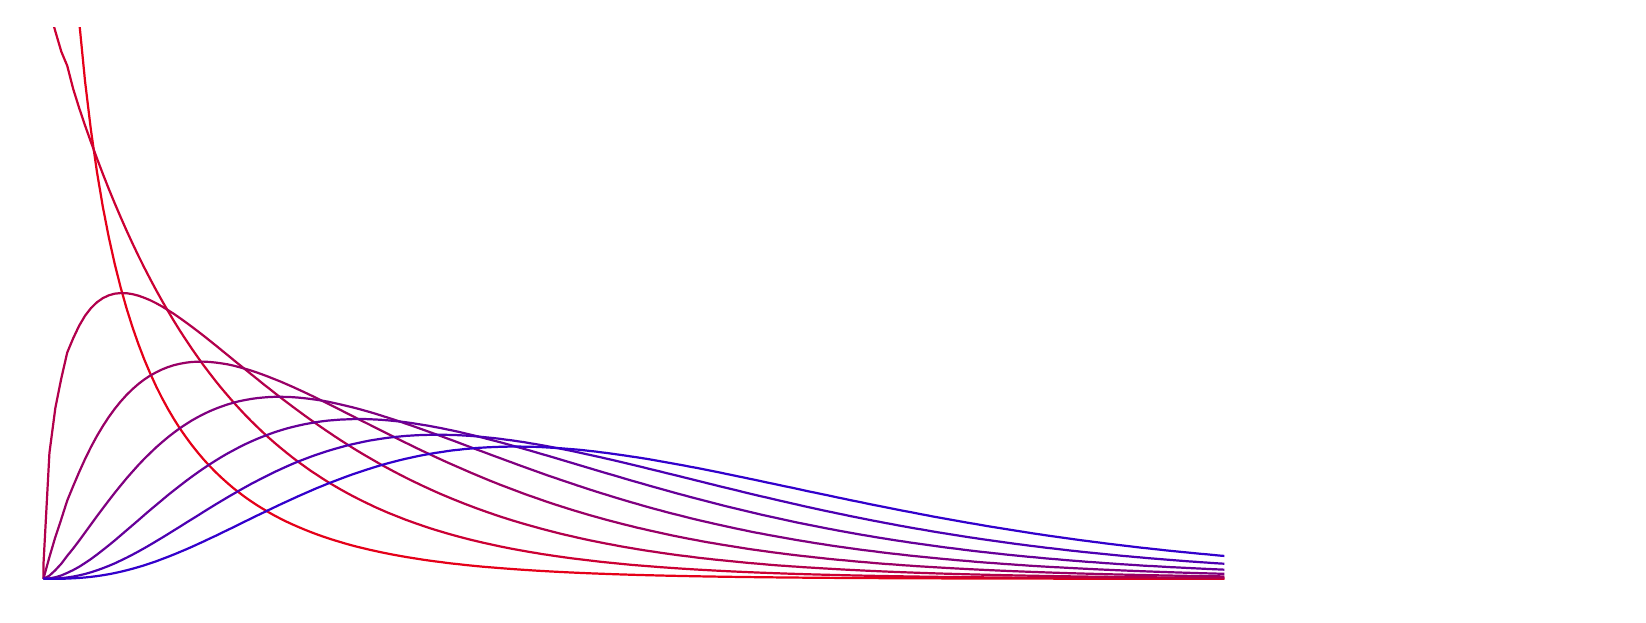
\begin{tikzpicture}[domain=.001:15,samples=200,thick]
    \clip (-0.2,-0.2) rectangle (20,7);
    \foreach[count=\k,evaluate={\z=\k>2?"(0,0)--":"";\c=10*\k}] 
      \g in {sqrt(pi),1,sqrt(pi)/2,1,3/4*sqrt(pi),2,15/8*sqrt(pi),6}
        \draw[color=blue!\c!red,yscale=15] \z 
          plot (\x,{exp(ln(\x/2)*\k/2-ln(\x)-\x/2-ln(\g))});
  \end{tikzpicture}
  % From a StackExchange question about plotting chi-squares in tikz
\end{frame}

\begin{frame}
  \frametitle{Degrees of Freedom}
  \begin{itemize}
    \item[] 
      (Variable 1 Categories - 1)(Variable 2 Categories - 1) 
      \vspace{0.5cm}
    \item[] 
      $(3-1)(2-1) = (2)(1) = 2$.
  \end{itemize}
\end{frame}

\begin{frame}
  \frametitle{$X$-squared distributions}
  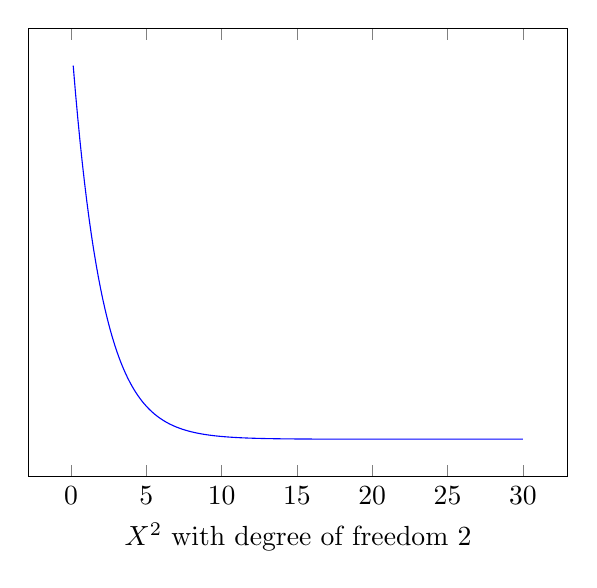
\begin{tikzpicture}
    \begin{axis}[
      ytick=\empty,
      xlabel=$X^2$ with degree of freedom 2,
    ]
    \addplot[
      domain=0:30,
      samples=200,
      color=blue,
    ]
    {exp(ln(x/2)-ln(x)-x/2)};
    \end{axis}
  \end{tikzpicture}
\end{frame}

\end{document}

